\section{App utenti}

\subsection{Introduzione e scopo del prodotto}
L'applicazione mobile è sviluppata per due diverse tipologie di utente ovvero il dipendente e l'addetto alle pulizie.

In generale offre all'utente le seguenti funzionalità:
\begin{itemize}
	\item \textbf{Login:} L'utente ha la possibilità di autenticarsi inserendo il proprio username e password; \\
	\item \textbf{Logout:} L'utente ha la possibilità di deautenticarsi premendo sull'elemento della lista "Logout" del menù principale in alto a destra. \\
\end{itemize}

Per quanto riguarda il dipendente, l'applicazione offre i seguenti servizi:
\begin{itemize}
	\item \textbf{Scansione:} Il dipendente ha la possibilità di scansionare una postazione per poter visualizzare lo stato di essa e altre informazioni come le prenotazioni associate a essa; \\
	\item \textbf{Occupazione:} Il dipendente dopo aver scansionato una postazione può occuparla se questa è prenotata da lui o è libera e igienizzata; \\
	\item \textbf{Igienizzare:} Il dipendente dopo aver scansionato una postazione la può igienizzare se questa risulta non igienizzata; \\
	\item \textbf{Lista prenotazioni:} Il dipendente può visualizzare le prenotazioni effettuate premendo sull'elemento della lista "Visualizza prenotazioni" del menù principale in alto a destra; \\
	\item \textbf{Disdire prenotazione:} Il dipendente può disdire una prenotazione dopo che è entrato nella pagina in cui visualizza tutte le prenotazioni effettuate; \\
	\item \textbf{Guida:} Il dipendente può visualizzare la guida premendo sull'elemento della lista "Guida" del menù principale in alto a destra; \\
	\item \textbf{Prenota postazione:} Il dipendente può prenotare una postazione premendo sull'elemento della lista "Prenota postazione" del menù principale in alto a destra.
	Dopo aver premuto dovrà inserire la data, l'ora di inizio, l'ora di fine e la stanza obbligatoriamente e in modo facoltativo anche il nome del collega.
	Una volta premuto sul bottone "Cerca", se è stato inserito il nome del collega, visualizzerà tutte le sue prenotazioni effettuate nella stanza, nel range orario e nella data inseriti e scorrendo sotto visualizzerà tutte le postazioni di quella stanza con il loro stato e potrà decidere quale prenotare se disponibile. \\	
\end{itemize}

\subsection{Requisiti e installazione}
	Per il corretto funzionamento l'app mobile richiede di essere installata su un dispositivo con sistema operativo Android con versione uguale o superiore alla 6.0 Marshmallow.
	
	\subsection{Utilizzo}
	L'applicazione mobile viene utilizzata dagli utenti che vogliono accedere a una postazione di una stanza dell'organizzazione. Essi hanno la possibilità di effettuare una prenotazione e di conoscere lo stato di una postazione, tramite la scansione del tag NFC associato. Inoltre per ogni occupazione viene registrato l'orario di inizio e di fine, e monitorata la presenza in tempo reale da parte dell'amministratore. Inoltre, ogni utente ha la possibilità di effettuare un'igienizzazione di una postazione precedentemente utilizzata. 
	\\All'utente dell'applicazione vengono offerte tutte le funzionalità indicate in questa sezione.
	\subsubsection{Login}
	\begin{figure}[H]
		\centering
		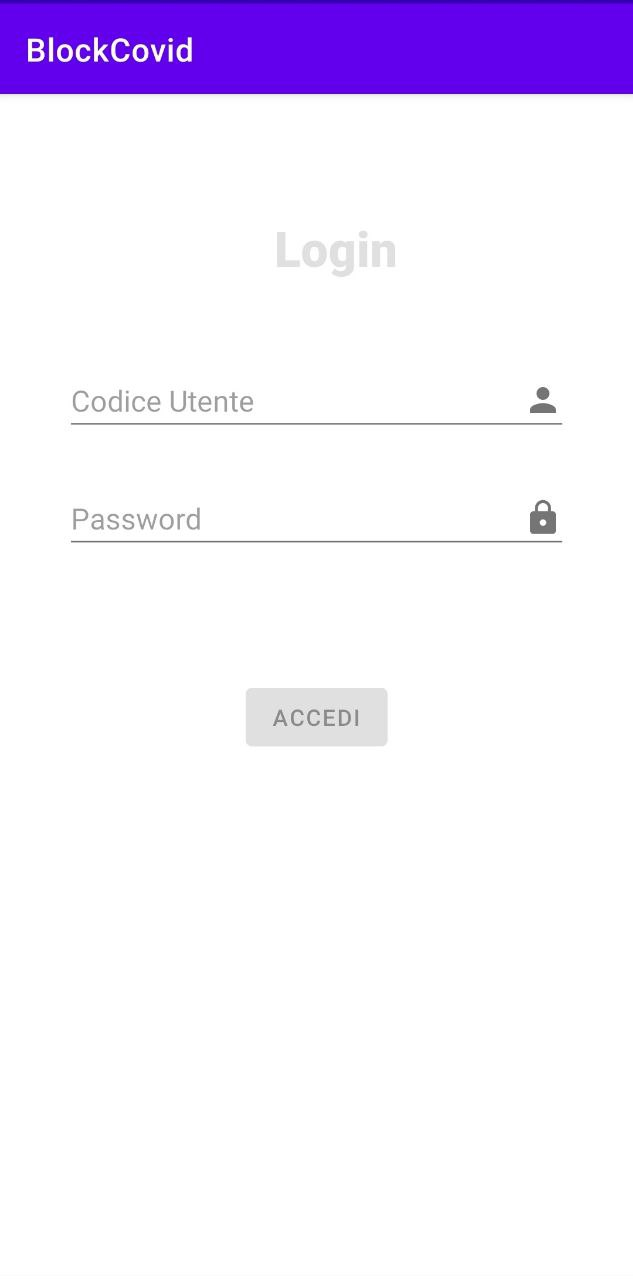
\includegraphics[width=5cm]{res/images/login.png}
		\caption{Login utente}
	\end{figure}
	L'utente può autenticarsi nella pagina del login inserendo il proprio username e la propria password nelle caselle di testo corrispondenti.
	Nel caso in cui inserisca le credenziali corrette otterrà l'accesso all'applicazione e quindi alla pagina principale, altrimenti verrà visualizzato un messaggio di errore in cui verrà comunicato di riprovare il login.
	
	\subsubsection{Logout}
	\begin{figure}[H]
		\centering
		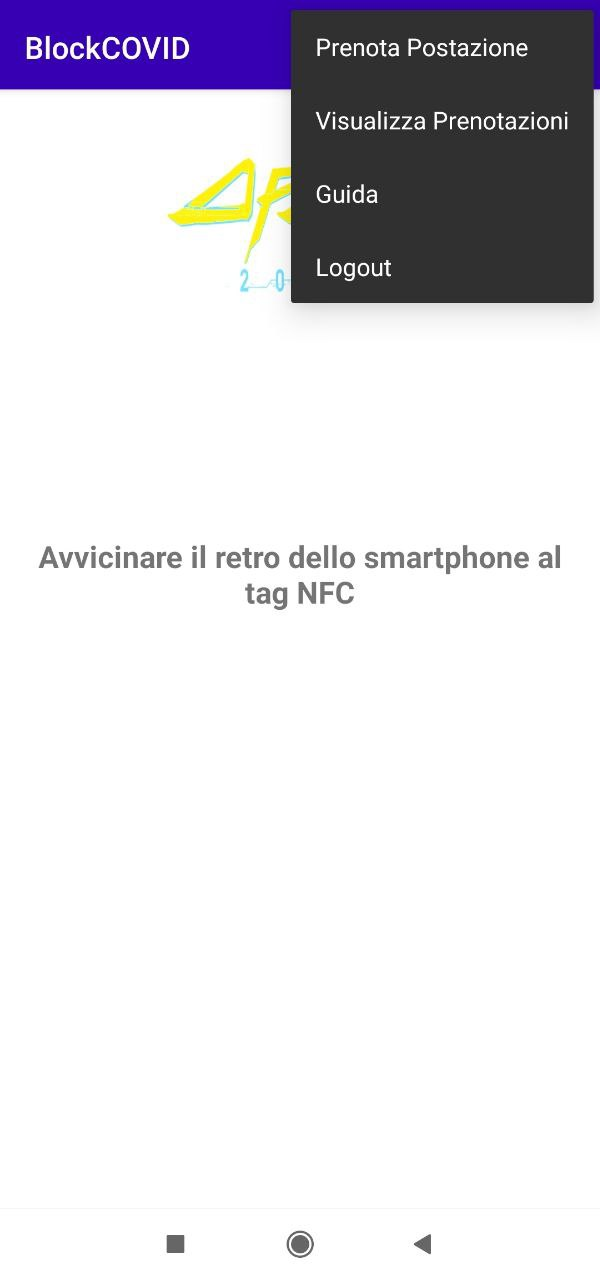
\includegraphics[width=5cm]{res/images/menuATendina.png}
		\caption{Logout utente}
	\end{figure}
	L'utente può eseguire il logout aprendo il menù a tendina in alto a destra e poi cliccando su logout. Avvenuta questa operazione l'utente sarà deautenticato dal sistema e si troverà nella pagina del login.
	
	\subsubsection{Scansione tag NFC}
	\begin{figure}[H]
		\centering
		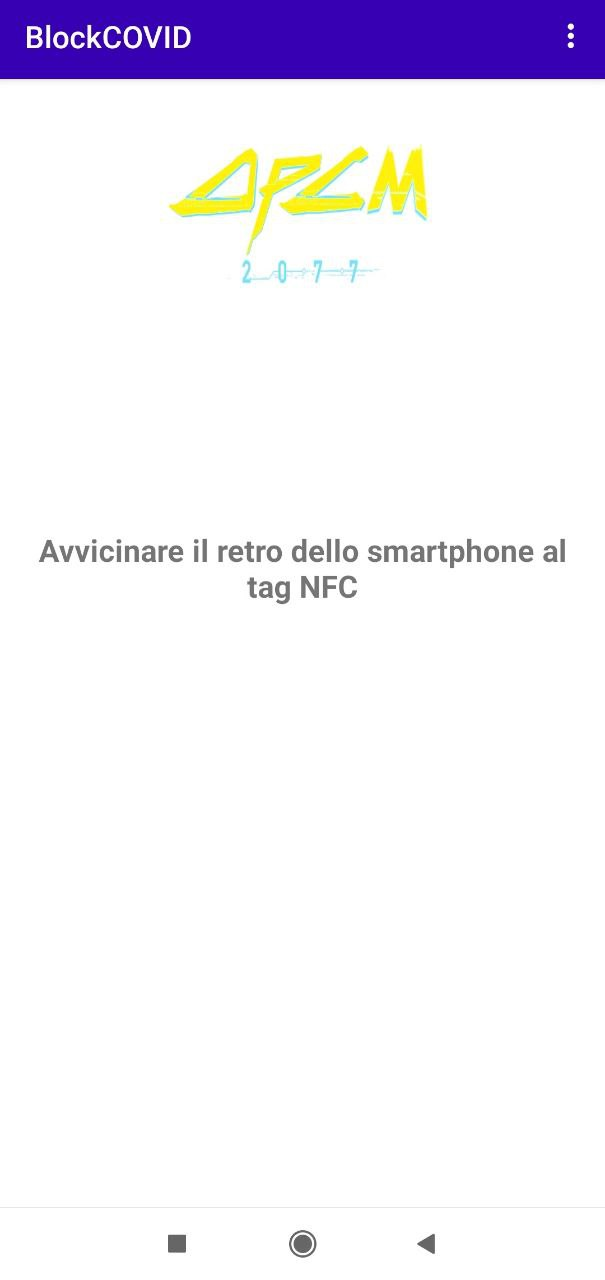
\includegraphics[width=5cm]{res/images/avvicinaSmartphone.png}
		\caption{Scansione tagNFC}
	\end{figure}
	L'utente si trova nella pagina principale dell'applicazione e gli viene chiesto di effettuare una scansione del tag NFC tramite lo smartphone per ottenere tutte le informazioni sulla postazione.
	\subsubsection{Visualizzazione stato postazione}
	\begin{figure}[H]
		\centering
		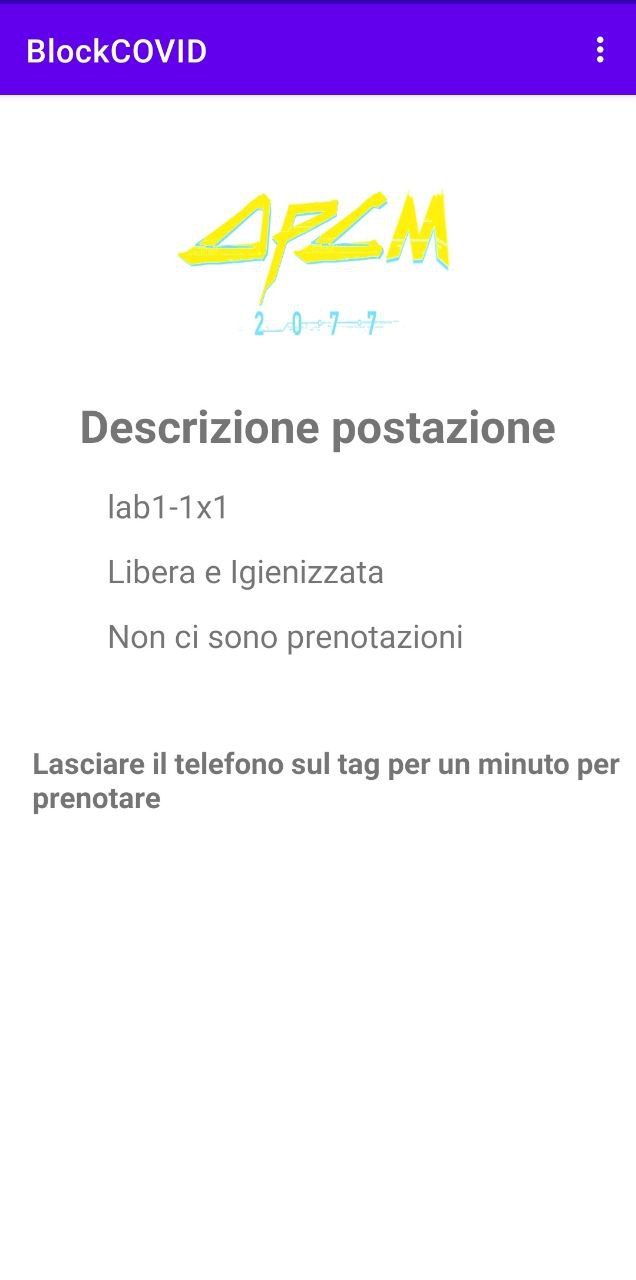
\includegraphics[width=5cm]{res/images/DescrizionePostazione1.png}
		\caption{Stato postazione}
	\end{figure}
	L'utente ha effettuato la scansione di una postazione e riceve le seguenti informazioni nella pagina principale dell'applicazione:
	\begin{itemize}
		\item stanza della prenotazione e posizione indicata tramite X e Y;
		\item stato della postazione;
		\item eventuale nome del dipendente che ha prenotato la postazione.
	\end{itemize}
	In base allo stato in cui si trova la postazione, l'utente visualizzerà un messaggio differente:
	\begin{itemize}
		\item se libera e igienizzata, si invita l'utente a lasciare il telefono sul tag NFC per effettuare una prenotazione automatica della postazione;
		\item se libera e non igienizzata, si invita l'utente a effettuare la pulizia autonoma della postazione tramite il kit aziendale e quindi di cliccare il bottone "igienizza", che modificherà lo stato in igienizzata;
		\item se prenotata e igienizzata, si invita l'utente ad abbandonare la postazione dato che al momento non è disponibile;
		\item se prenotata e non igienizzata, si invita l'utente a effettuare la pulizia autonoma della postazione tramite il kit aziendale e quindi di cliccare il bottone "igienizza", che modificherà lo stato in prenotata e igienizzata;
		\item se guasta e igienizzata, si invita l'utente ad abbandonare la postazione dato che al momento non è disponibile;
		\item se guasta e non igienizzata, si invita l'utente a effettuare la pulizia autonoma della postazione tramite il kit aziendale e quindi di cliccare il bottone "igienizza", che modificherà lo stato in guasta e igienizzata.
	\end{itemize}
	
	\subsubsection{Occupazione postazione}
	\begin{figure}[H]
		\centering
		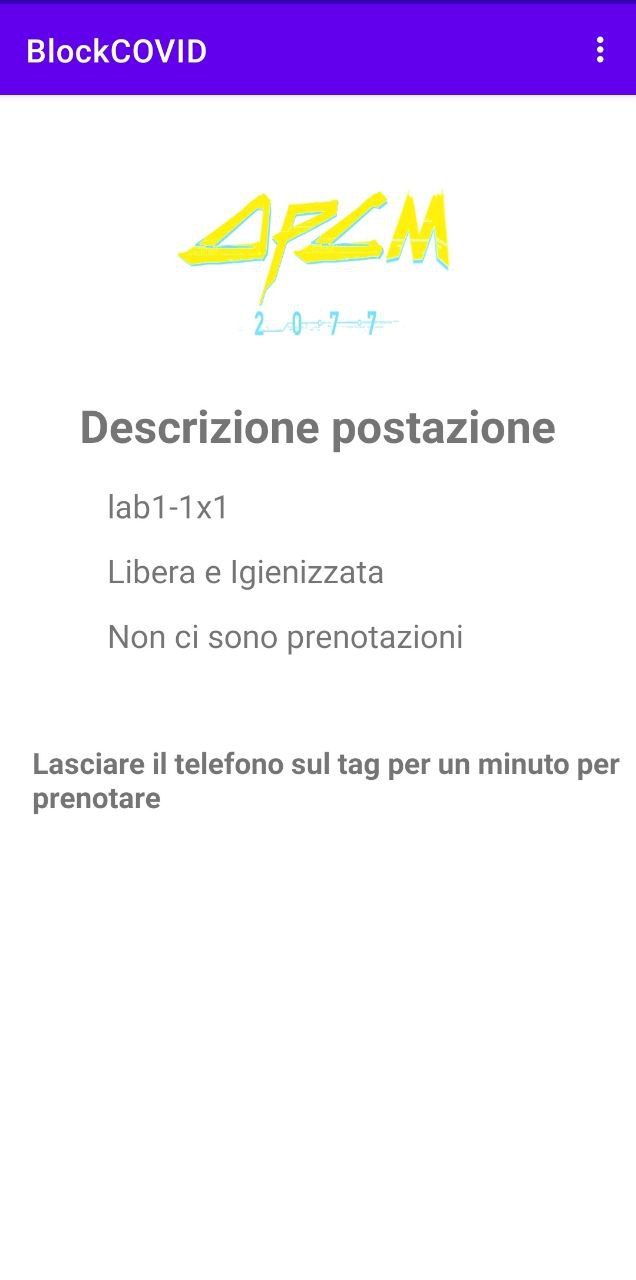
\includegraphics[width=5cm]{res/images/DescrizionePostazione1.png}
		\caption{Inizio occupazione postazione}
	\end{figure}
	L'utente dopo aver scansionato con il proprio smartphone il tag NFC per un tempo maggiore o uguale a un minuto, prenota in modo automatico la postazione per
	l’intera giornata lavorativa. Lo stato della postazione deve essere libera e igienizzata e non prenotata da un altro utente durante il resto della giornata.
	\subsubsection{Igienizzazione postazione}
	\begin{figure}[H]
		\centering
		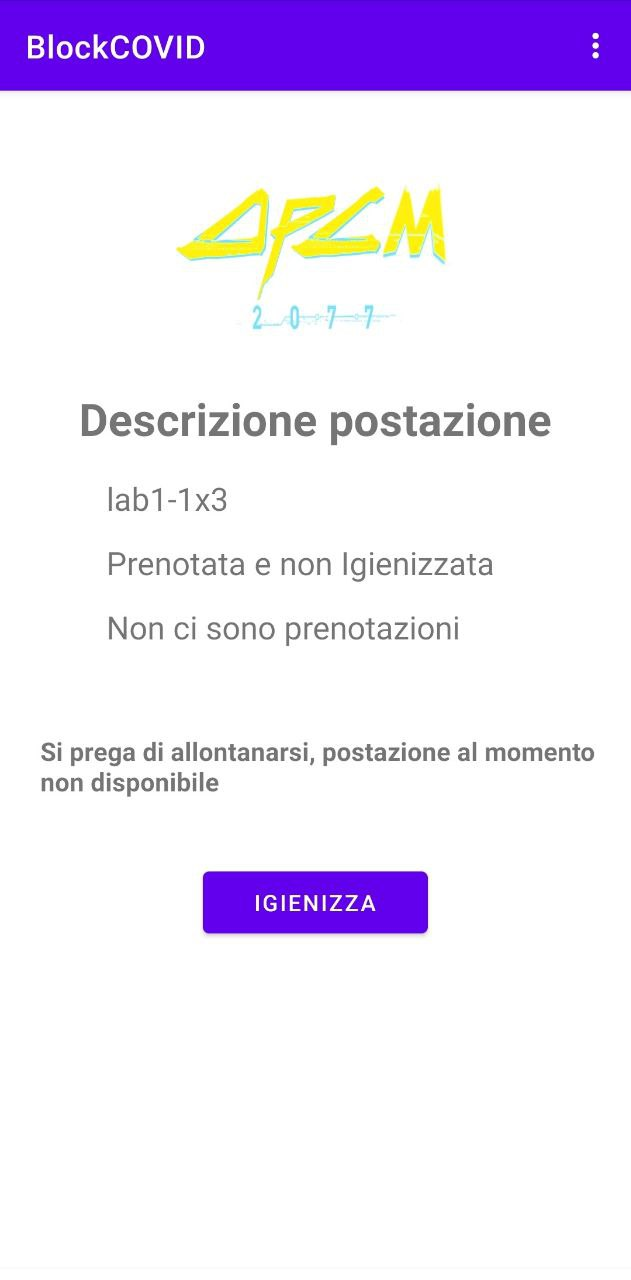
\includegraphics[width=5cm]{res/images/DescrizionePostazione3.png}
		\caption{Igienizzazione postazione}
	\end{figure}
	L'utente igienizza una postazione il cui stato è diverso da "igienizzato" e lo segnala premendo l'apposito bottone "igienizza" nella pagina principale dell'applicazione. In modo automatico lo stato della postazione viene registrato come libera e igienizzata, prenotata e igienizzata o guasta e igienizzata.
	\subsubsection{Visualizzazione lista prenotazioni}
	\begin{figure}[H]
		\centering
		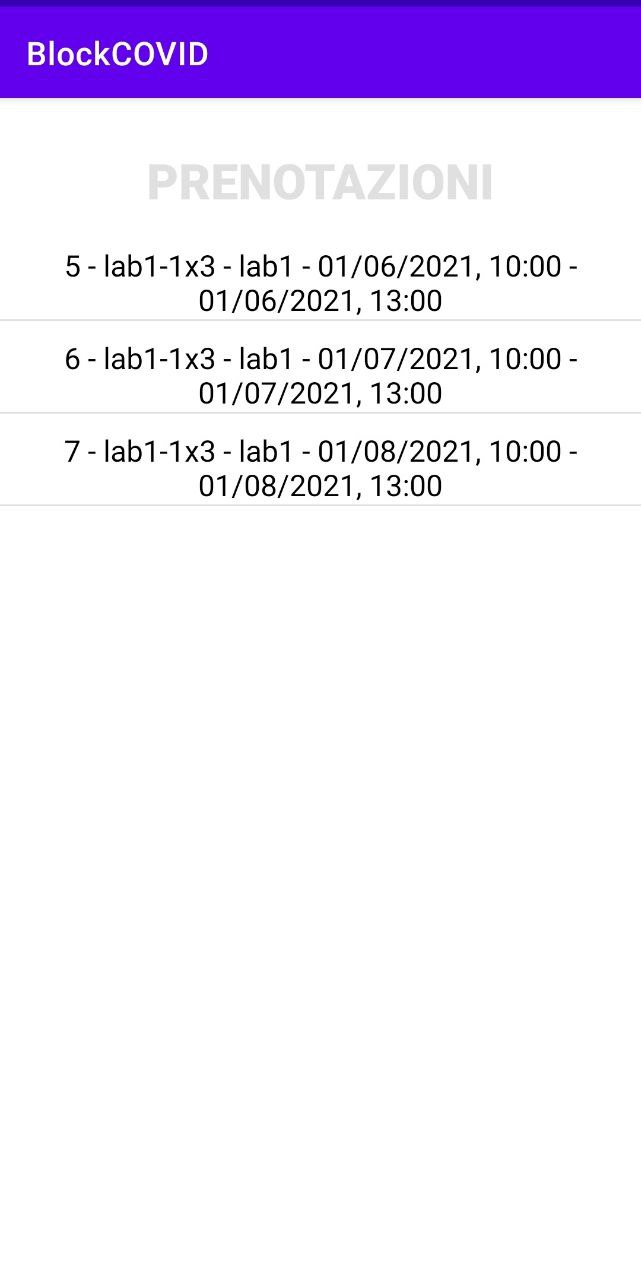
\includegraphics[width=5cm]{res/images/VisualizzaPrenotazioni.png}
		\caption{Visualizzazione lista prenotazioni}
	\end{figure}
	L’utente può accedere alla sezione per la visualizzazione della lista delle prenotazioni da lui effettuate cliccando nel menù a tendina in alto a destra "Visualizza prenotazioni".
	Ogni prenotazione mostra le seguenti informazioni:
	\begin{itemize}
		\item stanza della prenotazione;
		\item posizione indicata tramite X e Y;
		\item data di inizio della prenotazione;
		\item ora di inizio della prenotazione;
		\item data di fine della prenotazione;
		\item ora di fine della prenotazione.
	\end{itemize}
	\subsubsection{Disdetta prenotazione}
	\begin{figure}[H]
		\centering
		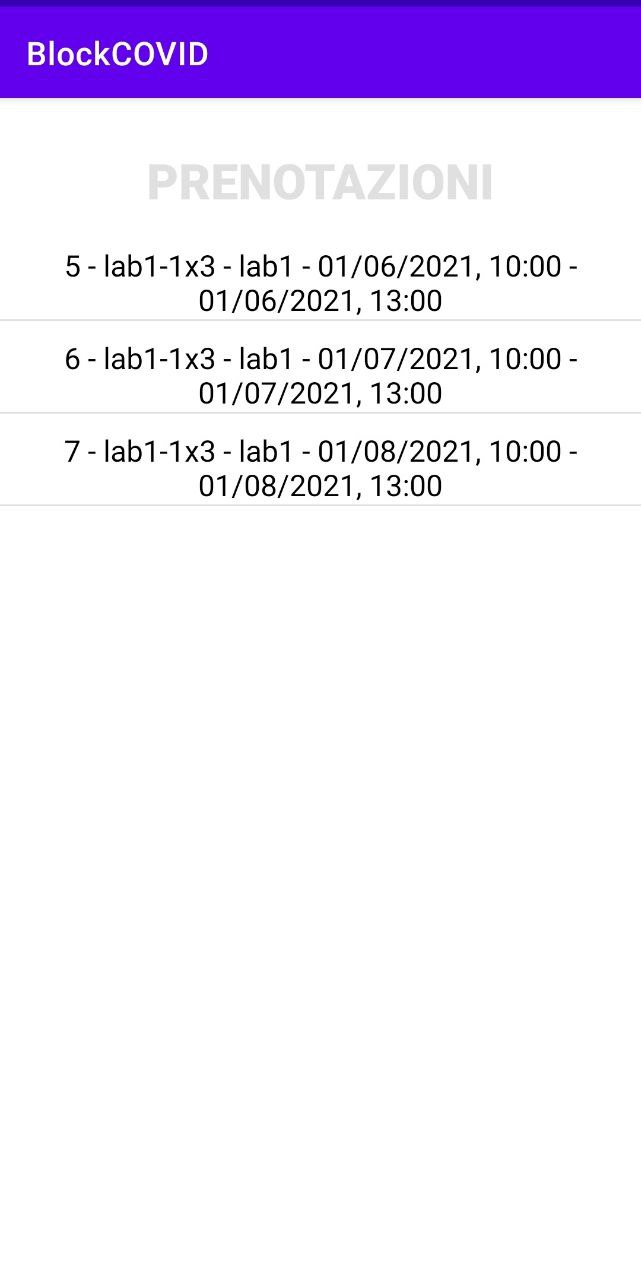
\includegraphics[width=5cm]{res/images/VisualizzaPrenotazioni.png}
		\caption{Disdetta prenotazione}
	\end{figure}
	L’utente si trova nella sezione di visualizzazione della lista delle prenotazioni, arrivatoci cliccando il menù a tendina in alto a destra, e disdice una prenotazione da lui effettuata in precedenza.
	\subsubsection{Guida utente}
	\begin{figure}[H]
		\centering
		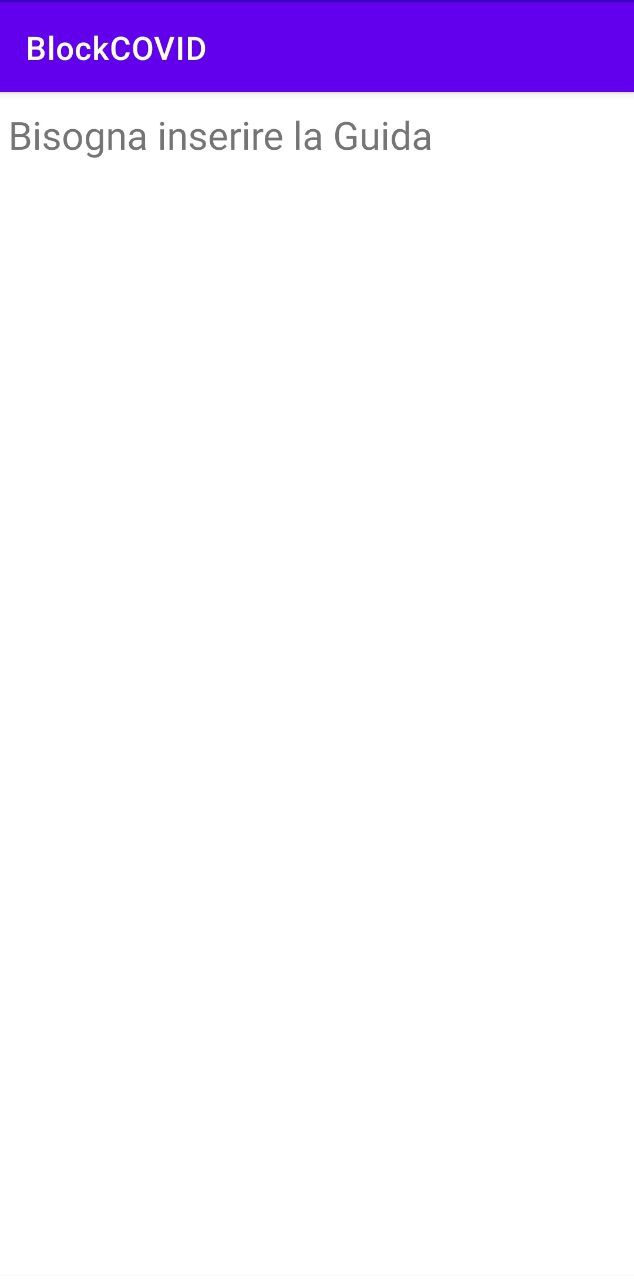
\includegraphics[width=5cm]{res/images/Guida.png}
		\caption{Guida dipendente}
	\end{figure}
	L’utente accede alla pagina Guida utente, cliccando la sezione apposita del menù a tendina in alto a destra, e riceve una guida riguardo le funzionalità principali dell'applicazione.
	\subsubsection{Prenotazione postazione}
	\begin{figure}[H]
		\centering
		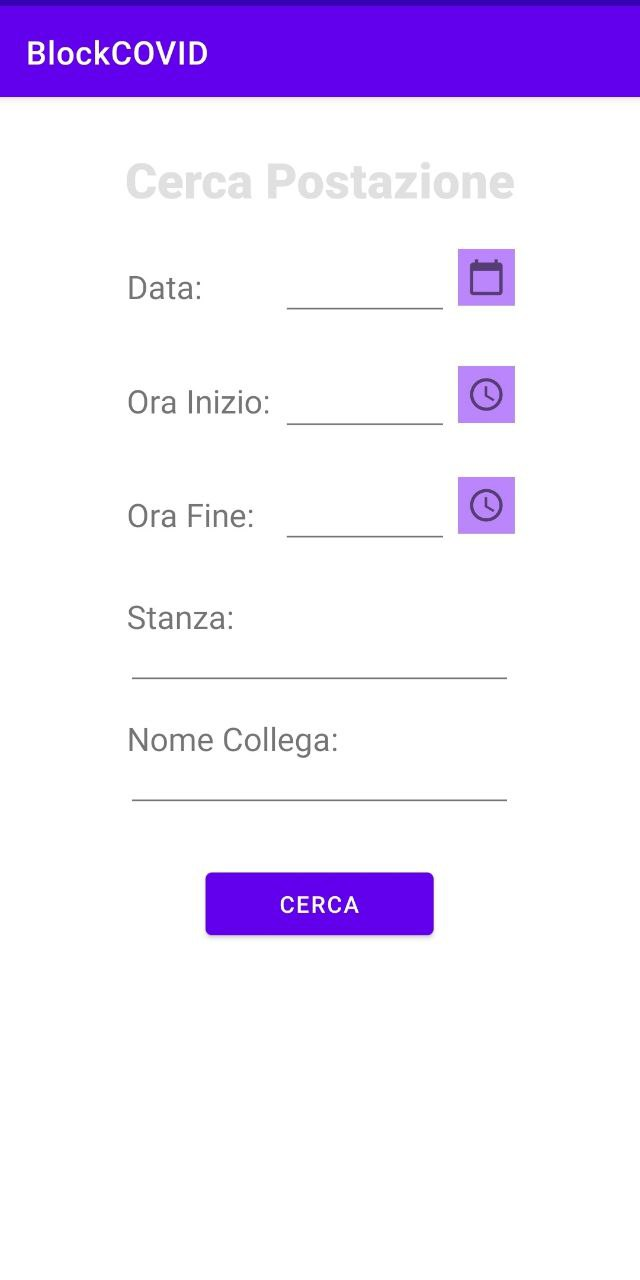
\includegraphics[width=5cm]{res/images/PrenotaPostazione.png}
		\caption{Prenotazione postazione}
	\end{figure}
	Il dipendente può prenotare una postazione premendo sull'elemento della lista "Prenota postazione" del menù principale in alto a destra.
	Dopo aver premuto dovrà inserire la data, l'ora di inizio, l'ora di fine e la stanza obbligatoriamente e in modo facoltativo anche il nome del collega. Per facilitare l'utente nell'inserimento dei dati, sono presenti una vista a calendario per la selezione di una data e una vista a orologio per la selezione di un orario. Una volta premuto sul bottone "Cerca", se è stato inserito il nome del collega, visualizzerà tutte le sue prenotazioni effettuate nella stanza, nel range orario e nella data inseriti e scorrendo sotto visualizzerà tutte le postazioni di quella stanza con il loro stato e potrà decidere quale prenotare se disponibile. 
	
	
